\documentclass[tikz,border=2pt]{standalone}
\usepackage{amsmath,amssymb}
\usepackage{pgfplots}
\pgfplotsset{compat=1.18}
\usetikzlibrary{arrows.meta}
\begin{document}
% Riley's ovens, mu = 2 per hour: E[W] against lambda for c = 1 (M/M/1: lambda/(mu(mu-lambda)))
% and c = 2 (M/M/2: E[Q]/lambda with E[Q] = 2 rho^3/(1-rho^2), rho = lambda/4); at lambda = 1.9: 9.5 and 0.146.
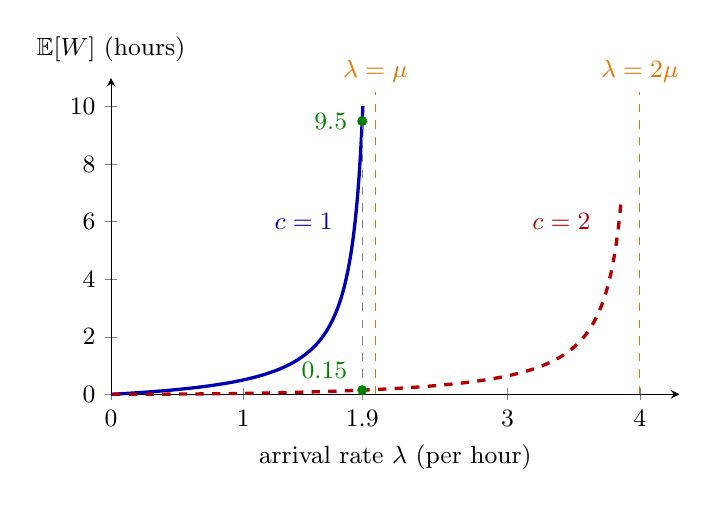
\begin{tikzpicture}[font=\small, >={Latex[length=2mm]}]
  \begin{axis}[
    axis lines=left, xmin=0, xmax=4.3, ymin=0, ymax=11,
    xtick={0,1,1.9,3,4}, xticklabels={$0$,$1$,$1.9$,$3$,$4$}, ytick={0,2,4,6,8,10},
    xlabel={arrival rate $\lambda$ (per hour)}, ylabel={$\mathbb{E}[W]$ (hours)},
    ylabel style={rotate=-90, anchor=south, at={(axis description cs:0,1.02)}},
    width=8.8cm, height=5.6cm, clip=false]
    \draw[orange!90!black, thin, dashed] (axis cs:2,0) -- (axis cs:2,10.5);
    \draw[orange!90!black, thin, dashed] (axis cs:4,0) -- (axis cs:4,10.5);
    \node[orange!90!black, anchor=south] at (axis cs:2,10.5) {$\lambda=\mu$};
    \node[orange!90!black, anchor=south] at (axis cs:4,10.5) {$\lambda=2\mu$};
    \addplot[blue!70!black, very thick, domain=0:1.905, samples=200] {x/(2*(2-x))};
    \addplot[red!70!black, very thick, dashed, domain=0.01:3.86, samples=200] {2*(x/4)^3/(1-(x/4)^2)/x};
    \node[blue!70!black, anchor=east] at (axis cs:1.75,6) {$c=1$};
    \node[red!70!black, anchor=east] at (axis cs:3.7,6) {$c=2$};
    \draw[gray, thin, dashed] (axis cs:1.9,0) -- (axis cs:1.9,9.5);
    \fill[green!50!black] (axis cs:1.9,9.5) circle (1.8pt);
    \fill[green!50!black] (axis cs:1.9,0.1457) circle (1.8pt);
    \node[green!50!black, anchor=east] at (axis cs:1.86,9.5) {$9.5$};
    \node[green!50!black, anchor=south east] at (axis cs:1.86,0.22) {$0.15$};
  \end{axis}
\end{tikzpicture}
\end{document}
